\documentclass{article}
\usepackage[catalan]{babel}
%\usepackage[latin1]{inputenc}   % Permet usar tots els accents i car�ters llatins de forma directa.
\usepackage[utf8]{inputenc} 
\usepackage{enumerate}
\usepackage{amsfonts, amscd, amsmath, amssymb}
\usepackage[pdftex]{graphicx}

\setlength{\textwidth}{16cm}
\setlength{\textheight}{24.5cm}
\setlength{\oddsidemargin}{-0.3cm}
\setlength{\evensidemargin}{0.25cm} \addtolength{\headheight}{\baselineskip}
\addtolength{\topmargin}{-3cm}

\newcommand\Z{\mathbb{Z}}
\newcommand\R{\mathbb{R}}
\newcommand\N{\mathbb{N}}
\newcommand\Q{\mathbb{Q}}
\newcommand\K{\Bbbk}
\newcommand\C{\mathbb{C}}

\newcounter{exctr}
\newenvironment{exemple}
{ \stepcounter{exctr} 
\hspace{0.2cm} 
\textit{Exemple  \arabic{exctr}: }
\it
\begin{quotation}
}{\end{quotation}}


\begin{document}

\textbf{\Large Tema 1. Introducci\'o al Processament Digital del Senyal.}

\vskip 0.2 cm
\noindent
\textbf{\large Senyals}

\vskip 0.2 cm
\noindent
Un \textbf{senyal} \'es el conjunt de valors num\`erics resultants de mesurar un 
fenomen f\'isic que varia amb el temps, l'espai o qualsevol altre par\`ametre.

\vskip 0.2 cm
\noindent
Exemples:
\begin{itemize}
\item La mesura del corrent el\`ectric que mostra un oscil.loscopi.
\item Les variacions de la pressi\'o de l'aire quan una persona parla.
\item Un electrocardiograma.
\item Una fotografia.
\end{itemize}

En aquest curs ens limitarem a estudiar els senyals que varien respecte a un \'unic par\`ametre,
que en general ser\`a el temps, per tant els senyals estaran formats per una 
\textit{seq\"u\`encia de valors}. 
En funci\'o de com siguin aquesta seq\"u\`encia i aquest conjunt de valors poder classificar els
senyals de la seg\"uent manera:

\vskip 0.5 cm

\begin{center}

\begin{tabular}{c|c|c|}
 & Seq\"u\`encia cont\'inua & Seq\"u\`encia discreta \\ & & \\ \hline  & & \\

\begin{tabular}{c}
Conjunt continu \\ \\
de valors 
\end{tabular}

&
  
\begin{tabular}{c}
Senyal Anal\`ogic 
\\ \\
\begin{minipage}{5cm}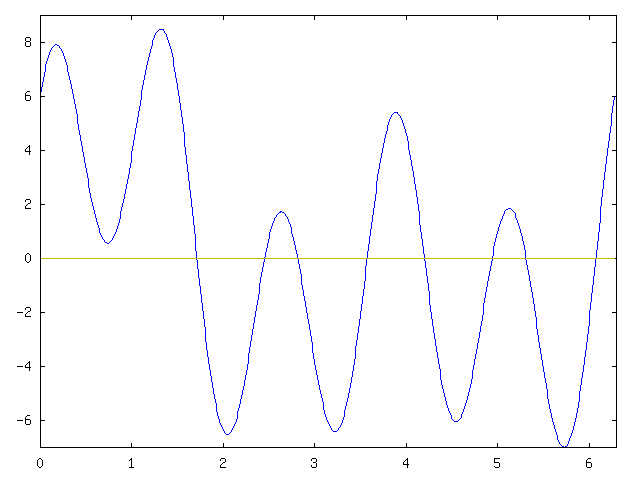
\includegraphics[width=5cm]{signalanalog.png}\end{minipage}
\end{tabular}

& 

\begin{tabular}{c}
Senyal en temps discret 
\\ \\
\begin{minipage}{5cm}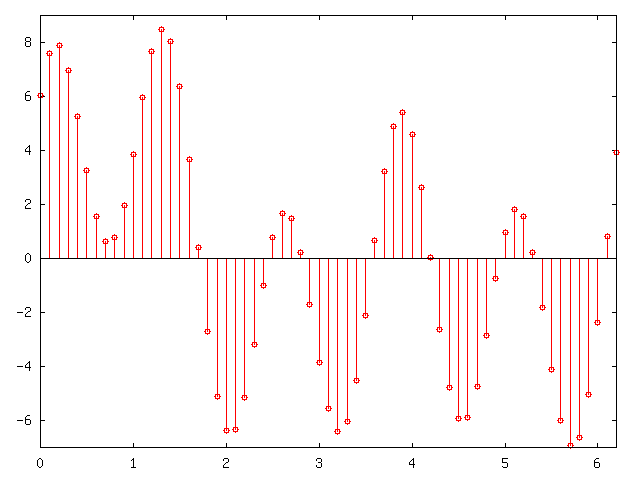
\includegraphics[width=5cm]{signaldisctime.png}\end{minipage}
\end{tabular}

\\ & & \\ \hline & & \\

\begin{tabular}{c}
Conjunt discret \\ \\
de valors 
\end{tabular}

 &

\begin{minipage}{5cm}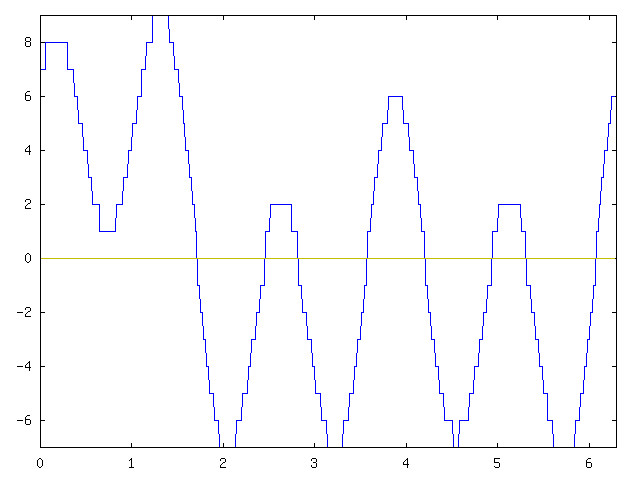
\includegraphics[width=5cm]{signaldiscvalues.png}\end{minipage}                 

& 

\begin{tabular}{c}
Senyal digital
\\ \\
\begin{minipage}{5cm}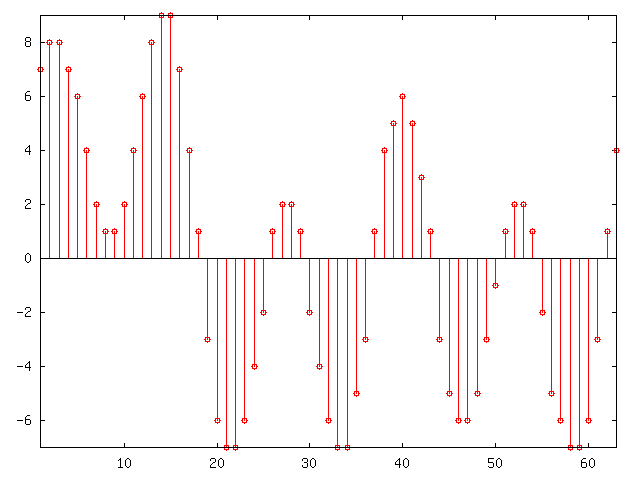
\includegraphics[width=5cm]{signaldigital.png}\end{minipage}
\end{tabular}

\\
\hline

\end{tabular}

\end{center}


\vskip 0.2 cm
\noindent
\textbf{Notaci\'o}

\vskip 0.2 cm
\noindent
Matem\`aticament els senyals es modelen com a funcions: $f: A \rightarrow B$, on els conjunts $A$ i $B$ 
depenen del tipus de senyal:

\vskip 0.3 cm

\begin{center}
\begin{tabular}{c|c|c|}
 & 
\begin{tabular}{c} Seq\"u\`encia cont\'inua \\ $A=\R$ \end{tabular}
 & 
\begin{tabular}{c} Seq\"u\`encia discreta \\ $A=\Z$ \end{tabular} 

\\ & & \\ \hline  & & \\

\begin{tabular}{c}
Conjunt continu \\ \\
de valors \\ \\
$B=\R$ o $B=\C$
\end{tabular}

& 

\begin{tabular}{c}
Senyal anal\`ogic \\ \\
Notaci\'o: $f(t)$ 
\end{tabular}

& 

\begin{tabular}{c}
Senyal en temps discret \\ \\
Notaci\'o: $f(nT)$ 
\end{tabular}

\\ & & \\ \hline  & & \\

\begin{tabular}{c}
Conjunt discret \\ \\
de valors \\ \\
$B=\{v_0, v_1, \cdots, v_k, \cdots \}$ \\ \\
on $v_i \in \R$ o $v_i \in \C$
\end{tabular}

& 


& 

\begin{tabular}{c}
Senyal digital \\ \\
Notaci\'o: $f[n]$ 
\end{tabular}

\\
\hline

\end{tabular}
\end{center}

\vskip 0.3 cm
\noindent
Si $B$ est\`a format per valors reals deim que el senyal \'es un \textbf{senyal real},
si est\`a format per valors complexes parlam de \textbf{senyal complexe}.


\vskip 0.5 cm
\noindent
\textbf{Tractament analògic vs. tractament digital de senyals}

Per \textbf{tractament o processament de senyal} entenem qualsevol operaci\'o que permet generar, rebre,
enviar o modificar un senyal. Fins als anys 60 la majoria de senyals amb qu\`e treballaven els enginyers eren 
senyals anal\`ogics (per exemple senyals de radar) que es tractaven amb circuits electr\`onics anal\`ogics 
(basats en v\`alvules i transistors). Amb l'aparici\'o dels ordinadors i els circuits digitals es va passar 
a treballar amb senyals digitals, que s\'on els \'unics que poden tractar els ordinadors.
L'\'us de la tecnologia digital permet molta m\'es flexibilitat en el tractament de senyals.
El \textbf{processament digital de senyals} fa refer\`encia a les modificacions que afecten els senyals digitals.

La figura \ref{filtreAnalogic} mostra un exemple d'un circuit electrònic (filtre analògic) que fa un processament d'un
senyal analògic. La figura \ref{filtreDigital} mostra l'exemple d'un programa d'ordinador (filtre digital) que fa
un filtratge equivalent. Resulta evident que és més senzill canviar els paràmetres del filtre digital modificant algunes
línees del codi que haver de remplaçar resistències i condensadors en el circuit digital.

\begin{figure}[htbp]
\centering
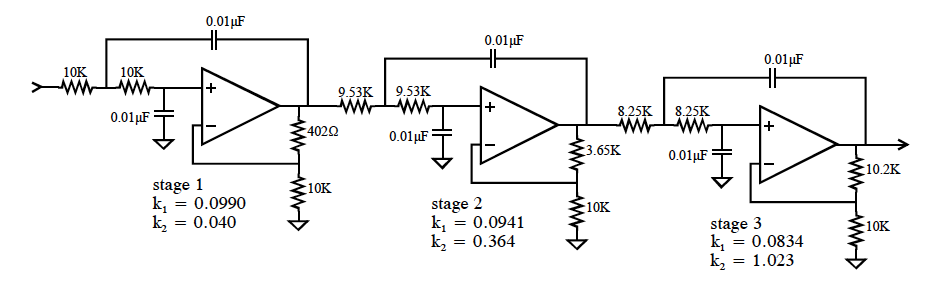
\includegraphics[width=14cm]{filtreanalogic.png} 
\caption{Exemple de filtre analògic (font: The Scientist and Engineer's Guide to Digital Signal Processing, A.W. Smith)}
\label{filtreAnalogic}
\end{figure}

\begin{figure}[htbp]
\centering
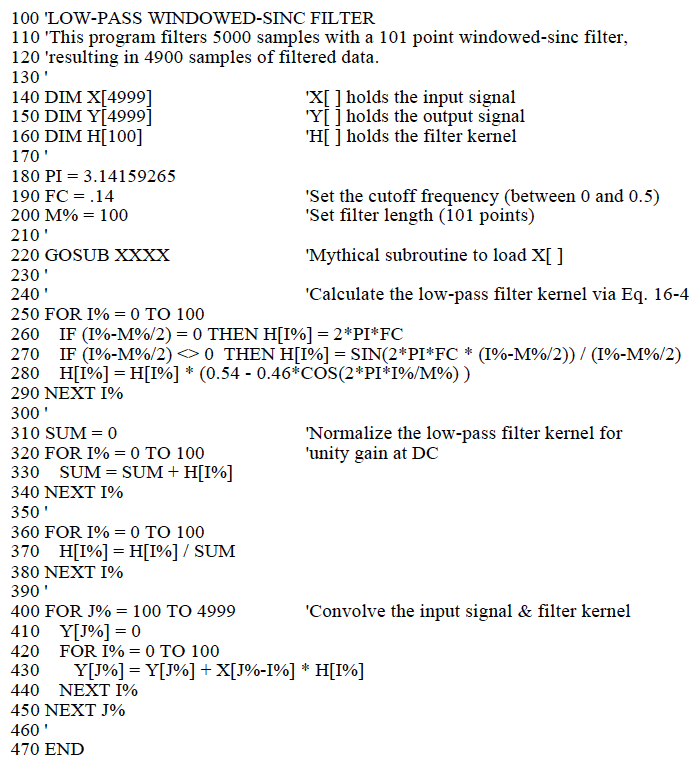
\includegraphics[width=12cm]{filtredigital.png} 
\caption{Exemple de filtre digital (font: The Scientist and Engineer's Guide to Digital Signal Processing, A.W. Smith)}
\label{filtreDigital}
\end{figure}

\vskip 0.3 cm
\noindent
\textbf{Conversi\'o anal\`ogica-digital}

\vskip 0.2 cm
\noindent
Per a que els filtres analògic i digital mostrats en les figures anteriors siguin realment equivalents
és necessari convertir primer els senyals d'entrada analògics a format digital. I, una vegada processats,
convertir la sortida a format analògic.
Un senyal anal\`ogic es pot transformar en digital mitjantzant la
\textbf{digitalitzaci\'o}, que compren un proc\'es de \textbf{mostreig}
i un proc\'es de \textbf{quantitzaci\'o} (veure figura \ref{conversioAD}). 
La conversi\'o inversa (de
digital a anal\`ogic) tamb\'e \'es possible i el senyal obtingut \'es
id\`entic a l'original sempre que la quantitzaci\'o i el mostreig 
verifiquin unes certes condicions.

\begin{figure}[htbp]
\centering
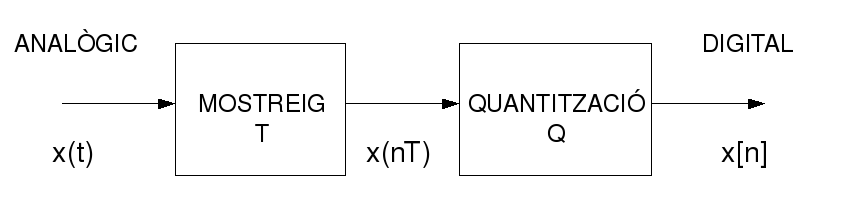
\includegraphics[width=14cm]{conversioAD.png} 
\caption{Conversi\'o anal\`ogica-digital}
\label{conversioAD}
\end{figure}

\newpage
\noindent
\textbf{\large Senyals digitals}

\vskip 0.2 cm
\noindent
En aquest curs treballarem principalment amb senyals digitals, els quals es poden 
descriure mitjan\c{c}ant una seq\"u\`encia de n\'umeros o mitjan\c{c}ant una f\`ormula.

\vskip 0.2 cm
\noindent
Exemples:
\begin{itemize}
\item $x[n]=\{ \cdots, 5, \underline{7}, 15, 11, \cdots \}$ (seq\"u\`encia infinita)
\item $x[n]=\{2, 9, \underline{-4}, -3, 5, 17 \}$  (seq\"u\`encia finita)
\item $x[n]=(-1)^n + 2$  (seq\"u\`encia infinita)
\end{itemize}

\vskip 0.2 cm
\noindent
\textbf{Alguns senyals importants}:
\begin{itemize}
\item \textbf{Delta de Dirac (impuls unitari)}: $\delta[n]=\begin{cases} 1 & \text{si } n=0 \\ \\ 0 & \text{altrament} \end{cases}$
\item \textbf{Esgla\'o unitari:} $u[n]=\begin{cases} 1 & \text{si } n \geq 0 \\ \\ 0 & \text{altrament} \end{cases}$
\item \textbf{Senyal sinuso\"idal}:
\[
x[n]=A \cos(\omega n + \theta) \qquad \quad  \text{o}  \qquad \quad x[n]=A \sin(\omega n + \theta)
\]

\noindent
$A$ s'anomena amplitud, $\omega$ \'es la freq\"u\`encia angular ($\omega=2\pi f$) i $\theta$ \'es
la fase del senyal.

\item \textbf{Senyal exponencial complexe}:
\[
x[n]=a^n , \qquad a \in \C
\]

\noindent
Observem que, donat que $a$ \'es un nombre complexe, llavors $a=r e^{i\theta}$ i per tant
\[
x[n]=a^n = r^n e^{i \theta n} = r^n (\cos(\theta n) + i \sin(\theta n)) = r^n \cos(\theta n) + i r^n \sin(\theta n)=x_R[n]+i x_I[n]
\]
\noindent
on $x_R$ i $x_I$ s\'on senyals sinuso\"idals.

\end{itemize}

\vskip 0.2 cm
\noindent
\textbf{Classificaci\'o dels senyals}. 

\vskip 0.2 cm
\noindent
Els senyals digitals es poden classificar seguint diversos
criteris:
\begin{itemize}
\item Senyals peri\`odics i no peri\`odics. El senyal $x[n]$ es diu \textbf{peri\`odic}
si verifica la seg\"uent condici\'o:
\[
x[n]=x[n+N] \qquad \forall n \in \Z \qquad \qquad \text{per a algun $N \in \Z$} 
\]
\item Senyals parells i senars.

\noindent
$x[n]$ \'es parell si $x[n]=x[-n]$

\noindent
$x[n]$ \'es senar o imparell si $x[n]=-x[-n]$

\vskip 0.2 cm
\noindent
Propietat: donat un senyal qualsevol $x[n]$, $x_P[n]=\frac{1}{2} (x[n]+x[-n])$ \'es
un senyal parell, $x_I[n]=\frac{1}{2} (x[n]-x[-n])$ \'es un senyal senar i, a m\'es,
$x[n]=x_P[n]+x_I[n]$.

\item Senyals d'energia i de pot\`encia.

\noindent
$x[n]$ \'es un \textbf{senyal d'energia finita} si 
\[
E=\sum_{-\infty}^{+\infty} |x[n]|^2 < \infty
\]

\noindent
$x[n]$ \'es un \textbf{senyal de pot\`encia finita} si 
\[
P=\lim_{N \rightarrow \infty} \frac{1}{2N+1} \sum_{-N}^{+N} |x[n]|^2 < \infty
\]

\item Senyals causals i anticausals.

\noindent
$x[n]$ \'es \textbf{causal} si $x[n]=0$ $\forall n < 0$

\noindent
$x[n]$ \'es \textbf{anticausal} si $x[n]=0$ $\forall n \geq 0$


\item Senyals deterministes i aleatoris. Els senyals \textbf{deterministes} s\'on aquells
els valors dels quals s\'on coneguts sense cap incertesa. 
Els senyals \textbf{aleatoris}, en canvi, evolucionen amb el temps d'una manera
impredictible. Aquest senyals es modelen com a \textbf{processos aleatoris}
que, en general, es consideren estacionaris i erg\`odics.
\end{itemize}


\vskip 0.5 cm
\noindent
\textbf{Operacions b\`asiques amb senyals}.
\begin{itemize}
\item Reflexi\'o ($R$). $y[n]=R \, x[n] = x[-n]$ 

\item Translaci\'o ($T_k$). $y[n]=T_k \, x[n] = x[n-k]$

\item Delmaci\'o ($D_k$). $y[n]=D_k \, x[n]=x[k n]$

\item Producte per un escalar. $y[n]=k \cdot x[n]$

\item Suma de senyals. $y[n]=x_1[n] + x_2[n]$

\item Producte de senyals. $y[n]=x_1[n] \cdot x_2[n]$
 
\end{itemize}

\vskip 0.2 cm
\noindent
Aquestes operacions es poden representar gr\`aficament mitjan\c{c}ant \textbf{diagrames de blocs}:

\vskip 0.4 cm
\begin{center}
\begin{tabular}{cc}
Reflexi\'o & Delmaci\'o \\
\begin{minipage}{5cm}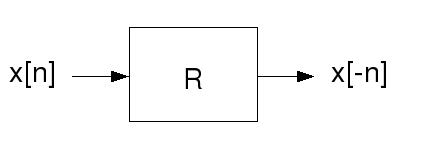
\includegraphics[width=5cm]{diagramareflexio.png}\end{minipage} & 
\begin{minipage}{5cm}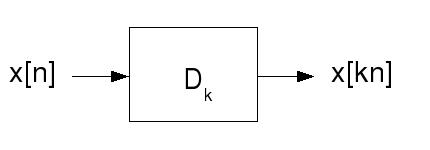
\includegraphics[width=5cm]{diagramadelmacio.png}\end{minipage}
\end{tabular}
\end{center}

\vskip 0.4 cm
\begin{center}
\begin{tabular}{cc}
Translaci\'o unit\`aria a la dreta & Translaci\'o unit\`aria a l'esquerra  \\
 (retard unitari) & (avan\c{c} unitari) \\
\begin{minipage}{5cm}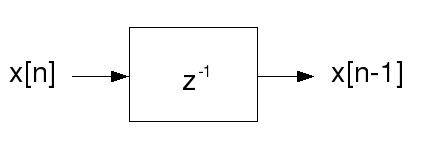
\includegraphics[width=5cm]{diagramaretard.png}\end{minipage} & 
\begin{minipage}{5cm}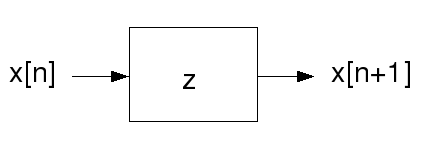
\includegraphics[width=5cm]{diagramaavanc.png}\end{minipage}
\end{tabular}
\end{center}

\vskip 0.4 cm
\begin{center}
\begin{tabular}{ccc}
Suma & Producte & Producte per escalar \\
\begin{minipage}{5cm}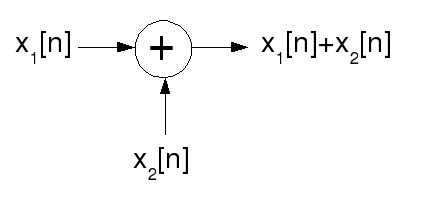
\includegraphics[width=5cm]{diagramasuma.png}\end{minipage} & 
\begin{minipage}{5cm}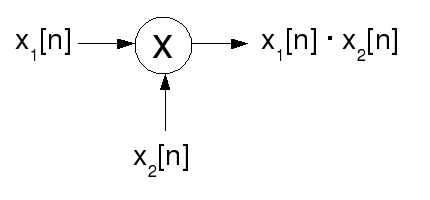
\includegraphics[width=5cm]{diagramaproducte.png}\end{minipage} & 
\begin{minipage}{5cm}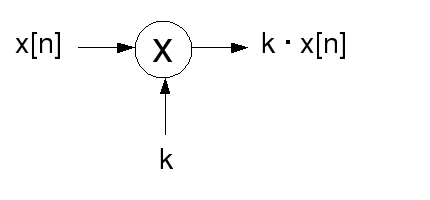
\includegraphics[width=5cm]{diagramaproducteesc.png}\end{minipage} 
\end{tabular}
\end{center}

\vskip 0.3 cm
\noindent
\textbf{Descomposici\'o d'un senyal en deltes de Dirac}

\vskip 0.2 cm
\noindent
Qualsevol senyal $x[n]$ es pot escriure com una combinaci\'o de deltes
de Dirac mitjan\c{c}ant les operacions de suma, producte per escalars i
translaci\'o, segons la f\`ormula seg\"uent:
\[
x[n]=\sum_{k=-\infty}^{+\infty} x[k] \delta[n-k]
\]


\vskip 0.3 cm
\noindent
\textbf{Convoluci\'o de senyals} 

\vskip 0.2 cm
\noindent
La convoluci\'o \'es una operaci\'o entre dos senyals que es denota amb el s\'imbol $*$
i es defineix de la seg\"uent manera:

\[
y[n]=x_1[n] * x_2[n]=\sum_{k=-\infty}^{+\infty} x_1[k] x_2[n-k] 
\]

\noindent
Propietats de la convoluci\'o:
\begin{itemize}
\item $x_1[n] * x_2[n] = x_2[n] * x_1[n]$
\item $x_1[n] * (x_2[n] * x_3[n])=(x_1[n] * x_2[n]) * x_3[n]$
\item $x_1[n] * (x_2[n] + x_3[n]) = x_1[n] * x_2[n] + x_1[n] * x_3[n]$
\item Si $x_1[n]$ t\'e una durada $M_1$ i $x_2[n]$ una durada $M_2$, llavors
$x_1[n] * x_2[n]$ t\'e una durada $M_1+M_2-1$.
\end{itemize}

\vskip 0.2 cm
\noindent
\textbf{Observaci\'o}: $x[n]=x[n] * \delta[n]$


\end{document}